%---------------------------------------------------------------------
\begin{frame}{Základní modely prostorové regrese}
\begin{itemize}
	\item \textbf{Prostorová autokorelace závislé proměnné}
	$$\bm{y}_t = \rho \bm{W}\bm{y}_t + \dots$$
	$\bm{Wy}_t$ popisuje prostorovou interakci mezi endogenními proměnnými modelu
	$\textit{SpatialLag}(y_{it}) = \bm{w}^T_i \bm{y}_t$, kde je $ \bm{w}^T_i$ řádek matice $\bm{W}$, $\bm{y}_t$ jsou pozorování $y$ v čase $t$.\\
	$\rho$ je koeficient prostorové autokorelace závislé proměnné (skalár); obvykle $\rho \in (-1,1)$.
	\item \textbf{Prostorová autokorelace regresorů}
	$$\bm{y}_t = \dots + \bm{X}_t \bm{\beta} + \bm{W}\bm{X}_t \bm{\theta} + \dots$$
	$\bm{X}$ je obvyklá matice regresorů, $\bm{WX}$ popisuje exogenní prostorové interakce mezi nezávislými proměnnými, $\bm{\beta}$ a $\bm{\theta}$ jsou vektory ($k\times 1$) neznámých parametrů, které se snažíme odhadnout.
\end{itemize}
\end{frame}
%---------------------------------------------------------------------
\begin{frame}{Základní modely prostorové regrese}
\begin{itemize}
	\item \textbf{Prostorová autokorelace náhodné složky} 
	$$\bm{u}_t = \lambda \bm{Wu}_t + \bm{\epsilon}_t$$
	 $\bm{Wu}_t$ popisuje prostorovou interakci mezi náhodnými složkami prostorových jednotek \\
	 $\lambda$ je koeficient prostorové autokorelace náhodné složky, resp. vynechaných prostorově  závislých vysvětlujících proměnných (skalár) \\
	 $\bm{\epsilon}_t$ vektor skutečných náhodných složek – prostorově nezávislá část náhodných složek.
	\item \textbf{Volba modelu se zahrnutím prostorové autokorelace} \\
		Konkrétní typ modelu volíme pomocí omezujících předpokladů: položíme $\rho,\theta$ nebo $\lambda$ rovné nule.
	Omezující předpoklady lze testovat. 
\end{itemize}
\end{frame}
%---------------------------------------------------------------------
\begin{frame}{Základní modely prostorové regrese}
\textbf{Spatial lag model}
\begin{itemize}
	\item Zajímá-li nás prostorová interakce mezi pozorovanými hodnotami závislé proměnné. Prostorovou závislost (strukturu) zde předpokládáme pouze u endogenní proměnné modelu. Model, resp. jeho redukovaná forma, mají tvar: 
	\begin{align*}
	\bm{y}_t & = \rho \bm{Wy}_t + \bm{X}_t\bm{\beta}+ \bm{u}_t\\
	(\bm{I} - \rho \bm{W}) \bm{y}_t & = \bm{X}_t \bm{\beta} + \bm{u}_t
	\end{align*}
	\item Koeficienty $\rho$ i $\bm{\beta}$ jsou odhadnuty metodou maximální věrohodnosti (MLE). Koeficienty  $\bm{\beta}$  pomáhají vysvětlit tu část variability $\bm{y}$, která není vysvětlena prostorově.	
\end{itemize}
\end{frame}
%---------------------------------------------------------------------
\begin{frame}{Základní modely prostorové regrese}
\textbf{Spatial Durbin model}
\begin{itemize}
	\item Vznikne rozšířením specifikace Spatial lag model o prostorové interakce mezi regresory: 
		\begin{align*}
		\bm{y}_t & = \rho \bm{Wy}_t + \bm{X}_t\bm{\beta}+ \bm{Wy}_t\bm{X}_t\bm{\theta} +  \bm{u}_t\\
		(\bm{I} - \rho \bm{W}) \bm{y}_t & = \bm{X}_t \bm{\beta} + \bm{Wy}_t\bm{X}_t\bm{\theta}+ \bm{u}_t
		\end{align*}
\end{itemize}
\end{frame}
%---------------------------------------------------------------------
\begin{frame}{Základní modely prostorové regrese}
\textbf{Spatial error model}
	\begin{align*}
	\bm{y}_t & =   \bm{X}_t\bm{\beta}+  \bm{u}_t, \qquad \bm{u}_t = \lambda  \bm{Wu}_t + \bm{\epsilon}_t\\
	\bm{y}_t & = \bm{X}_t\bm{\beta}+ \lambda\bm{Wy}_t\bm{u}_t+  \bm{\epsilon}_t\\
	(\bm{I} - \lambda \bm{W}) \bm{y}_t & = (\bm{I} - \lambda \bm{W}) \bm{X}_t \bm{\beta} + \bm{\epsilon}_t
	\end{align*}
\begin{itemize}

	\item I v případě, kdy se nezajímáme o prostorové interakce mezi pozorovanými proměnnými, můžeme zlepšit vlastnosti odhadu pomocí prostorově závislých chyb.
	\item Interakce v rámci náhodné složky nevyžadují teoretické zdůvodnění interakčního procesu, předpokládáme existenci prostorově závislých proměnných, nezahrnutých do modelu
\end{itemize}
\end{frame}
%---------------------------------------------------------------------
\begin{frame}{Prostorové modely:  stacionarita/stabilita}
\textbf{Stacionarita}
\begin{itemize}
\item Neformálně: pro každou oblast je počet sousedících oblastí omezený (malý)
\item Řádkové (a sloupcové) součty matice $\bm{S}$ jsou konečné a omezené, i když počet uvažovaných prostorových jednotek $n$ roste neomezeně.
\item Korelace mezi dvěma prostorovými jednotkami konverguje k nule s rostoucí vzdáleností mezi těmito jednotkami.
\item Formální podmínky stacionarity (pro $\rho, \lambda$ a $\bm{W}$ ) viz \href{https://www.google.cz/url?sa=t&rct=j&q=&esrc=s&source=web&cd=1&cad=rja&uact=8&ved=0ahUKEwjjwvLCk8bLAhXEvXIKHWSHBxsQFgggMAA&url=http://www.springer.com/cda/content/document/cda_downloaddocument/9783642403392-c2.pdf?SGWID\%3D0-0-45-1432965-p175381976&usg=AFQjCNGpme8ofJQzd46BCJVsUEio6oKIzQ&sig2=LlarV9wYhELGcTPiqzfRgg}{Elhorst (2014)}.
\end{itemize}
\end{frame}
%---------------------------------------------------------------------
\begin{frame}{Prostorové modely:  stacionarita/stabilita}
\textbf{Stabilita odhadů}
\begin{itemize}
	\item Matice $\bm{S}$, resp. matice $\bm{W}$ není odhadována, musíme ji stanovit předem. Odhadnuté koeficienty $\bm{\beta}$, resp. $\bm{\theta}$ závisejí na zvolené matici $\bm{W}$.
	\item "Řešení": regresní modely odhadujeme opakovaně, pokaždé s trochu jinak definovanou maticí $\bm{W}$ a porovnáváme vlastnosti jednotlivých odhadů.
    \item Tento postup zaručuje pouze lokální optimum (určíme nejlepší z porovnávaných modelů podle zvoleného kritéria), nikoliv globální optimum.
	\end{itemize}
\end{frame}
%---------------------------------------------------------------------
\section{Přímé a nepřímé efekty (Spill-overs)}
\begin{frame}{Přímé a nepřímé efekty (Spill-overs)}
\begin{itemize}
	\item $(\bm{I} - \rho \bm{W}) \bm{y}_t = \bm{X}_t \bm{\beta} + \bm{W}\bm{X}_t\bm{\theta} + \alpha \bm{\iota} +\bm{u}_t$ \quad $ \alpha \bm{\iota}$ je vektor úroňových konstant
	\item $\bm{y}_t = (\bm{I} - \rho \bm{W})^{-1} (\bm{X}_t\bm{\beta} + \bm{W}\bm{X}_t \bm{\theta})+ \bm{R}_t$ \quad 
	$\bm{R}_t$ obsahuje náhodnou složku i intercept 
\end{itemize}
Derivaci $E(\bm{y}_t)$ podle $k$-té vysvětlující proměnné $\bm{x}_{kt}$ lze zapsat jako:\\(časový index $t$ pro jednuduchost vynecháme)

\begin{align*} \bigg[\frac{\partial E(\bm{y})}{\partial \bm{x}_{1,k}} \dots \frac{\partial E(\bm{y})}{\partial \bm{x}_{N,k}}\bigg] & =
\begin{bmatrix}
\frac{\partial E(y_1)}{\partial \bm{x}_{1,k}} & \dots & \frac{\partial E(y_1)}{\partial \bm{x}_{N,k}} \\
\vdots & \ddots & \vdots \\
\frac{\partial E(y_N)}{\partial \bm{x}_{1,k}} & \dots & \frac{\partial E(y_N)}{\partial \bm{x}_{N,k}}
\end{bmatrix} = \\
& = (\bm{I} - \rho \bm{W})^{-1} 
\begin{bmatrix}
\beta_k & w_{12}\theta_k & \dots & w_{1N}\theta_k \\
w_{21}\theta_K & \beta_k & \dots & w_{2N}\theta_k \\
\vdots & \ddots & \ddots & \vdots \\
w_{N1}\theta_k & w_{N2}\theta_k & \dots & \beta_k 
\end{bmatrix}
\end{align*}
\end{frame}
%---------------------------------------------------------------------
\begin{frame}{Přímé a nepřímé efekty (Spill-overs)}
$$ \bigg[\frac{\partial E(\bm{y})}{\partial \bm{x}_{1,k}} \dots \frac{\partial E(\bm{y})}{\partial \bm{x}_{N,k}}\bigg] =
 (\bm{I} - \rho \bm{W})^{-1} 
\begin{bmatrix}
\beta_k & w_{12}\theta_k & \dots & w_{1N}\theta_k \\
w_{21}\theta_K & \beta_k & \dots & w_{2N}\theta_k \\
\vdots & \ddots & \ddots & \vdots \\
w_{N1}\theta_k & w_{N2}\theta_k & \dots & \beta_k 
\end{bmatrix}
$$
%---------------------------------------------------------------------
\begin{itemize}
	\item Změním-li hodnotu vysvětlující proměnné $x_k$ u $i$-té prostorové jednotky (změna $x_{ik}$), dojde ke změně očekávané hodnoty $y_i$ - \textbf{přímý efekt} a zároveň dojde ke změně očekávané hodnoty $y$ u dalších prostorových jednotek – \textbf{nepřímý efekt}. 
	\item Diagonální prvky matice (RHS) představují přímé efekty, prvky mimo diagonálu jsou nepřímé efekty
\end{itemize}

\end{frame}
%---------------------------------------------------------------------
\begin{frame}{Přímé a nepřímé efekty (Spill-overs)}
$$ \bigg[\frac{\partial E(\bm{y})}{\partial \bm{x}_{1,k}} \dots \frac{\partial E(\bm{y})}{\partial \bm{x}_{N,k}}\bigg] =
(\bm{I} - \rho \bm{W})^{-1} 
\begin{bmatrix}
\beta_k & w_{12}\theta_k & \dots & w_{1N}\theta_k \\
w_{21}\theta_K & \beta_k & \dots & w_{2N}\theta_k \\
\vdots & \ddots & \ddots & \vdots \\
w_{N1}\theta_k & w_{N2}\theta_k & \dots & \beta_k 
\end{bmatrix}
$$

\begin{itemize}
	\item Přímé a nepřímé efekty se liší pro jednotlivé prostorové jednotky ($i$).
	\begin{itemize}
	\item 	Přímé efekty se liší, protože diagonální prvky $(\bm{I} - \rho \bm{W})^{-1} $ jsou různé, pokud $\rho \neq 0$.
	\item Nepřímé efekty se liší, protože prvky mimo diagonálu matice $\bm{W}$, resp. $(\bm{I} - \rho \bm{W})^{-1}$ jsou různé, pokud $\rho \neq 0$ a/nebo $\theta_k \neq 0$
\end{itemize}
	$$ (\bm{I} - \rho \bm{W})^{-1} = \bm{I} + \rho\bm{W} + \rho^2\bm{W}^2 + \rho^3\bm{W}^3 + \dots$$

	\item Diagonální prvky matice (RHS) představují přímé efekty, prvky mimo diagonálu jsou nepřímé efekty
\end{itemize}
\end{frame}
%---------------------------------------------------------------------
\begin{frame}{Přímé a nepřímé efekty (Spill-overs)}
$$ \bigg[\frac{\partial E(\bm{y})}{\partial \bm{x}_{1,k}} \dots \frac{\partial E(\bm{y})}{\partial \bm{x}_{N,k}}\bigg] =
(\bm{I} - \rho \bm{W})^{-1} 
\begin{bmatrix}
\beta_k & w_{12}\theta_k & \dots & w_{1N}\theta_k \\
w_{21}\theta_K & \beta_k & \dots & w_{2N}\theta_k \\
\vdots & \ddots & \ddots & \vdots \\
w_{N1}\theta_k & w_{N2}\theta_k & \dots & \beta_k 
\end{bmatrix}
$$
%---------------------------------------------------------------------
\begin{itemize}
\item \textbf{Interpretace odhadnutého prostorového regresního modelu – vždy na základě přímých a nepřímých efektů}. 
\item Koeficient $\beta_k$ nepopisuje chování závislé proměnné $y_i$ při změně $x_{ik}$ "správně".
\item Statistickou významnost přímých efektů můžeme testovat viz \href{https://www.google.cz/url?sa=t&rct=j&q=&esrc=s&source=web&cd=1&cad=rja&uact=8&ved=0ahUKEwjjwvLCk8bLAhXEvXIKHWSHBxsQFgggMAA&url=http://www.springer.com/cda/content/document/cda_downloaddocument/9783642403392-c2.pdf?SGWID\%3D0-0-45-1432965-p175381976&usg=AFQjCNGpme8ofJQzd46BCJVsUEio6oKIzQ&sig2=LlarV9wYhELGcTPiqzfRgg}{Elhorst (2014)}.	
\end{itemize}
\end{frame}
%---------------------------------------------------------------------
\begin{frame}{Přímé a nepřímé efekty (Spill-overs)}
\begin{itemize}
	\item Ukázkový výstup odhadu přímých a nepřímých efektů (LeSage/Pace, 2009):
	$$\bm{y} = (\bm{I} - \rho \bm{W})^{-1} \bm{X}\bm{\beta} + (\bm{I} - \rho \bm{W})^{-1} \bm{\epsilon}$$
	$\dots$ jednoduchá regrese $y$ na $x$, použita prostorová regrese: \\
	Spatial lag model.
	
	\end{itemize}
\begin{table}[]
\centering
\caption{Spatial partitioning of direct, indirect and total   impacts}
\begin{tabular}{llll}
&         &          &             \\
                                                                                                       & Mean    & Std. dev & t-statistic \\
Direct effect                                                                                          & 0.586   & 0.0148   & 39.6106     \\
Indirect effect                                                                                        & 1.08414 & 0.0587   & 18.4745     \\
Total effect                                                                                           & 1.67    & 0.0735   & 22.7302    
\end{tabular}
\end{table}
\end{frame}
%---------------------------------------------------------------------
\begin{frame}{Přímé a nepřímé efekty (Spill-overs)}

$$ \bigg[\frac{\partial E(\bm{y})}{\partial \bm{x}_{1,k}} \dots \frac{\partial E(\bm{y})}{\partial \bm{x}_{N,k}}\bigg] =
(\bm{I} - \rho \bm{W})^{-1} 
\begin{bmatrix}
\beta_k & w_{12}\theta_k & \dots & w_{1N}\theta_k \\
w_{21}\theta_K & \beta_k & \dots & w_{2N}\theta_k \\
\vdots & \ddots & \ddots & \vdots \\
w_{N1}\theta_k & w_{N2}\theta_k & \dots & \beta_k 
\end{bmatrix}
$$
\begin{itemize}
	\item \textbf{Nevýhody, omezení modelů založených na prostorové závislosti:}
	\item Poměr přímého a nepřímého efektu nezávisí na $\beta_k$ - je dán pouze na základě matice $\bm{W}$ a hodnoty $\rho$. 
	\item Tento poměr je stejný pro všechny vysvětlující proměnné (resp. příslušné přímé a nepřímé efekty).
\end{itemize}

\end{frame}
%---------------------------------------------------------------------

\section{Prostorová regrese v R}
\begin{frame}{Prostorová regrese v R}
\begin{itemize}
	\item Knihovna \{spdep\} 
	\begin{itemize}
		\item Různé typy prostorových modelů
		\item Testy prostorové nezávislosti, identifikace prostorových shluků,$\dots$
	\end{itemize}
	\item	Knihovna \{splm\}
	\begin{itemize}
		\item Prostorová regrese na panelových datech
	\end{itemize}
	\item Knihovna \{ggplot2\} + další nutné knihovny
	\begin{itemize}
		\item Kartogramy (infomapy) / choropleth maps
	\end{itemize}
\end{itemize}
 \begin{figure}
 	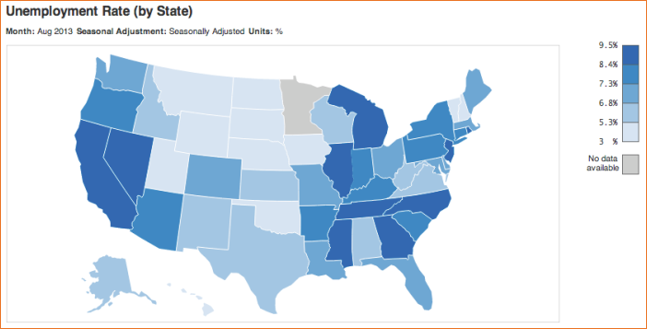
\includegraphics[width=.5\textwidth]{IMG/sp_unemp.PNG}
 \end{figure}

\end{frame}

%---------------------------------------------------------------------